\itemhead{复习题一 · 第17题（教材p.30）}{XJ-B1-C01-RV-P030-Y1286}
\label{XJ-B1-C01-RV-P030-Y1286}
{\footnotesize 湘教版教材p.30 / PDF第37页 / 复习题一 / 第17题}
\field{原题}{画出以方程 $(y-x)(y-x^2)=0$ 的解为坐标的所有点组成的图象。}
\field{参考答案}{图象为直线 $y=x$ 与抛物线 $y=x^2$ 的并，交点为 $(0,0),(1,1)$；并集图形本身不一定是一个函数的图象。}
\begin{center}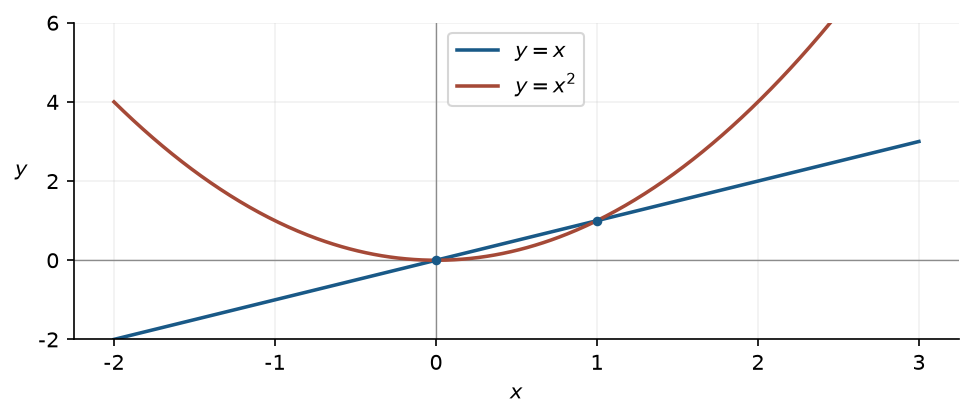
\includegraphics[width=.84\linewidth,height=.38\textheight,keepaspectratio]{figures/C01-RV030-17.png}\end{center}
{\small \field{关联知识}{S04 交集、并集及解集的联系（教材帮p.19、20 / PDF28、29）；F04 函数三种表示法、图象与读数（教材帮p.85、86、93、94 / PDF94、95、102、103）}
\field{方法与易错点}{先各自化简集合或解出约束，再在数轴上合并；有序数对交集通过联立方程求得。 易错：并集重复写元素；连接处一个闭端点也误删；把交集当并集。}
\field{答案依据}{答案册相关题组：PDF第8、9页（册内页7、8）；按当前题库原题逐项重算，不按旧版题号机械对套。}}
